\documentclass[12pt]{article}
\usepackage[pdftex,dvipsnames]{color}
\usepackage{graphicx}
\usepackage{amsmath}
\usepackage{amsfonts}
\newcommand{\eps}{\varepsilon}
\newcommand{\abso}[1]{\;\mid#1\mid\;}
\renewcommand{\=}{\,=\,}
\newcommand{\+}{\,+\,}
% ----------------------------------------------------------------
\newcommand{\remark}[1]{\par\noindent{\color[named]{ProcessBlue}#1}\par}
\newcommand{\mcc}[2]{\multicolumn{#1}{c}{#2}}
\newcommand{\mcp}[2]{\multicolumn{#1}{c|}{#2}}
\newcommand{\nm}[1]{\textsf{\small #1}}
\newcommand{\nnm}[1]{\textsf{\small\textit{#1}}}
\newcommand{\nmm}[1]{\nnm{#1}}

% no labels in list of references:
\makeatletter
\renewcommand\@biblabel{}
\makeatother

\hyphenation{Snij-ders Duijn DataSpecification dataspecification dependentvariable ModelSpecification}

% centered section headings with a period after the number;
% sans serif fonts for section and subsection headings
\renewcommand{\thesection}{\arabic{section}.}
\renewcommand{\thesubsection}{\thesection\arabic{subsection}}
\makeatletter
 \renewcommand{\section}{\@startsection{section}{1}
                {0pt}{\baselineskip}{0.5\baselineskip}
                {\centering\sffamily} }
 \renewcommand{\subsection}{\@startsection{subsection}{2}
                {0pt}{0.7\baselineskip}{0.3\baselineskip}
                {\sffamily} }
 \renewcommand{\subsubsection}{\@startsection{subsubsection}{3}
                {0pt}{0.7\baselineskip}{0.3\baselineskip}
                {\sffamily} }
\makeatother


\renewcommand{\baselinestretch}{1.0} %% For line spacing.
\setlength{\parindent}{0pt}
\setlength{\parskip}{1ex plus1ex}
\raggedright
\begin{document}

\title{Class Design for Siena 4}
\author{Krists Boitmanis}
\date{September 8, 2009}
\maketitle

\section{Introduction}

The purpose of this document is to give an overview of the C++ code for Siena 4.
Some notes:
\begin{itemize}
\item Names in the code are indicated as \nnm{name}.
\item Typewriter font is used for file names, like \texttt{FileName.cpp}.
\item Normally, a class named \nnm{SomeName} is declared in
the file \texttt{SomeName.h} and implemented in the file \texttt{SomeName.cpp}.
\item Camel case is used for names of classes, methods, and variables. More
specifically, all names but class names start with a lower case letter, and
when the name consists of several words, each of the subsequent words starts
with an upper case letter. Examples:
	\begin{itemize}
	\item \nnm{StatisticCalculator} -- a class name
	\item \nnm{calculateNetworkRateStatistics} -- a method name
	\item \nnm{observationCount} -- a variable name
	\end{itemize}
\item The names of pointer variables start with a `p' followed by an upper case
letter, like \nnm{pNetworkData}.
\item Similarly, the names of reference variables start with an `r', like in the
following declarations of a copy constructor and an assignment operator:
\begin{verbatim}
Network(const Network & rNetwork);
Network & operator=(const Network & rNetwork);
\end{verbatim}
\item Moreover, the names of instance variables are prepended with an `l', e.g.
	\begin{itemize}
	\item \verb|int| \nnm{lobservationCount} -- an instance variable of a
non-pointer type,
	\item \nnm{Model} * \nnm{lpModel} -- an instance variable of a pointer
type.
	\end{itemize}
\end{itemize}

\section{Library Overview}

The code is organised into libraries that correspond to the directory names
under \texttt{src}. The libraries are briefly explained in the following list
in the order of their dependencies, namely, no library depends on any other
library listed after it.
\begin{itemize}
\item \texttt{utils} -- contains various general purpose classes and functions.
\item \texttt{network} -- contains the classes \nnm{Network} and
\nnm{OneModeNetwork} for storing and manipulating directed two-mode and one-mode
networks, respectively, as well as supporting classes like various iterators
over ties in a network.
\item \texttt{data} -- contains everything related to the observed data
with the class \nnm{Data} being the main container storing the observations of
network and behavior variables, covariates, etc.
\item \texttt{model} -- contains the tools for specifying and simulating
actor-oriented models. The \nnm{Model} class can be used to specify an
actor-oriented model, which can be subsequently simulated with respect to a
specific \nnm{Data} object by using an instance of the \nnm{EpochSimulation}
class. Finally, the \nnm{StatisticCalculator} class provides the means for
calculating the observed or simulated statistics for effects in the model.
\end{itemize}

In the next sections, each library is explained in some detail.

\section{Utils}

\begin{itemize}
\item \texttt{Utils.h} provides miscellaneous utility functions, macros, and
classes.
\item \texttt{Random.h} provides functions for drawing random numbers.
\item The class \nnm{NamedObject} acts as a base class for anything that has
a name.
\item The singleton class \nnm{SqrtTable} is used throughout the system to
calculate square roots of integers efficiently. Once the root of an integer is
calculated, it is stored in a table for later reuse.

Example:
\begin{verbatim}
SqrtTable * pTable = SqrtTable::instance();
double root2 = pTable->sqrt(2);
\end{verbatim}
\end{itemize}

\section{Networks}

\subsection{\nnm{Network} class}

The \nnm{Network} class implements directed two-mode networks with
valued ties. The number of tie senders $n$ and the number of tie receivers $m$
have to be provided at the construction of a network. Technically,
the \nnm{Network} class can be used for storing one-mode networks as well,
in which case $n=m$, however, the derived class \nnm{OneModeNetwork} is
recommended for this purpose.

\subsubsection{Internal Data Representation}

The outgoing ties of each sender $i$ are stored in an STL (C++ Standard Template
Library) \nnm{map}. The alters of non-zero ties from $i$ act as keys in the map,
and the tie values are stored in the map as values corresponding to those keys.
The maps themselves are stored in an array \nnm{lpOutTies}, hence the value
of a tie $(i,j)$ can be accessed as
\nnm{lpOutTies}[\nnm{i}][\nnm{j}]. Similarly, an array
of maps \nnm{lpInTies} is used to store the incoming ties of all receivers.

While being much more memory efficient than storing the adjacency matrix
of a network explicitly, this representation still provides fast queries of
tie values -- the number of steps necessary to retrieve the value of a tie
$(i,j)$ is proportional to the logarithm of the out-degree of $i$. Also, this
representation directly provides a fast and convenient way of iterating over
all non-zero ties of an actor in the increasing order of the alters.

The users of the \nnm{Network} class should not care about its internal
representation, though, and use the public interface methods, to which we now
turn.

\subsubsection{Interface}

Some of the more important methods of the \nnm{Network} class are explained
in the following list.

\begin{itemize}
\item \nnm{Network}(\verb|int| \nnm{n}, \verb|int| \nnm{m}) -- constructs a
network with $n$ senders, $m$ receivers, and no ties.
\item \verb|int| \nnm{n}() -- returns the number of actors in the set of tie
senders.
\item \verb|int| \nnm{m}() -- returns the number of actors in the set of tie
receivers.
\item \verb|void| \nnm{setTieValue}(\verb|int| \nnm{i}, \verb|int| \nnm{j},
\verb|int| \nnm{v}) -- sets the specified value of the tie $(i,j)$.
\item \verb|int| \nnm{tieValue}(\verb|int| \nnm{i}, \verb|int| \nnm{j}) --
returns the value of the tie $(i,j)$.
\item \nnm{TieIterator} \nnm{ties}() -- returns an iterator over all ties of the
network. The ties are ordered according to their senders from smallest to
largest, and the ties from the same sender are ordered according to their
receivers.

Usage:
\begin{verbatim}
TieIterator iter = pNetwork->ties();

while (iter.valid())
{
  int ego = iter.ego();
  int alter = iter.alter();
  int value = iter.value();

  cout << "The tie from " << ego << " to " << alter <<
    " has a value " << value << endl;

  // Move on to the next tie
  iter.next();
}
\end{verbatim}

\item \nnm{IncidentTieIterator} \nnm{outTies}(\verb|int| \nnm{i}) -- returns
an iterator over the outgoing ties of actor $i$ in the increasing order of the
alters.

Usage:
\begin{verbatim}
IncidentTieIterator iter = pNetwork->outTies(i);

while (iter.valid())
{
  int alter = iter.actor();
  int value = iter.value();

  cout << "The tie from " << i << " to " << alter <<
    " has a value " << value << endl;

  // Move on to the next tie
  iter.next();
}
\end{verbatim}

\item \nnm{IncidentTieIterator} \nnm{inTies}(\verb|int| \nnm{i}) -- returns
a similar iterator over the incoming ties of actor $i$.
\item \verb|int| \nnm{outDegree}(\verb|int| \nnm{i}) -- returns the number of
non-zero outgoing ties for actor $i$.
\item \verb|int| \nnm{inDegree}(\verb|int| \nnm{i}) -- returns the number of
non-zero incoming ties for actor $i$.
\end{itemize}

\subsection{Iterators}

We have already seen the usage of supporting classes \nnm{TieIterator} and
\nnm{IncidentTieIterator}. Another iterator class, namely
\nnm{CommonNeighborIterator}, provides convenient means for iterating over
actors that are common to two instances of \nnm{IncidentTieIterator}. For
example, one can iterate over reciprocated ties of an actor in a one-mode
network as follows:
\begin{verbatim}
CommonNeighborIterator iter(pNetwork->inTies(i),
  pNetwork->outTies(i));

while (iter.valid())
{
  int neighbor = iter.actor();
  cout << "There is a reciprocated tie from " << i <<
    " to " << neighbor << endl;

  // Move on to the next neighbor
  iter.next();
}
\end{verbatim}

\subsection{\nnm{OneModeNetwork} class}

A one-mode network can be thought of as a special case of a two-mode network,
where the set of tie senders coincides with the set of tie receivers. Hence,
the \nnm{OneModeNetwork} class is derived from the \nnm{Network} class. In
addition to the interface inherited from the base class, it maintains the number
of reciprocated ties per each actor and provides various methods for counting
two-paths in a network. A non-exhaustive list of methods follows:

\begin{itemize}
\item \nnm{OneModeNetwork}(\verb|int| \nnm{n},
\verb|bool| \nnm{loopsPermitted}) -- constructs an empty network for $n$ actors.
Ties from actors to themselves (which are called loops) can be explicitly
forbidden by providing the value \verb|false| as the second argument.
\item \verb|int| \nnm{reciprocalDegree}(\verb|int| \nnm{i}) -- returns the
number of reciprocated ties of actor $i$.
\item \nnm{CommonNeighborIterator} \nnm{reciprocatedTies}(\verb|int| \nnm{i}) --
returns an iterator over all reciprocated ties of actor $i$. The usage is
similar to that of the method \nnm{Network}::\nnm{outTies}(\verb|int| \nnm{i})
except that the class \nnm{CommonNeighborIterator} does not have a \nnm{value}()
method. In a sense, the network is treated as a boolean network, where the
existence/non-existence of ties is of interest, but not the actual values of
ties.
\item \verb|int| \nnm{twoPathCount}(\verb|int| \nnm{i}, \verb|int| \nnm{j}) --
returns the number of two-paths from actor $i$ to actor $j$.
\end{itemize}

\section{Observed Data}

The \texttt{data} library contains classes for storing the observed data subject
to actor-oriented modeling. The entire set of observed data for a Siena project
(or one group in a multi-group project) should be stored in an instance of the
\nnm{Data} class. It owns collections of more specific data objects like those
storing the observed data for dependent network variables, constant actor
covariates, etc. This section will guide you step-by-step through the process of
populating a \nnm{Data} object. To begin with, an instance of the \nnm{Data}
class should be created:
\begin{verbatim}
int observationCount = 4;
Data * pData = new Data(observationCount);
\end{verbatim}
Note that the number of observations has to be provided in the very beginning.

\subsection{Actor Sets}

There may be several sets of actors involved, like a set of students, a
set of teachers, and a set of courses, therefore, when specifying dependent
variables and covariates, one should be explicit about the relevant actor sets.
Each set of actors is represented in the system by an instance of the
\nnm{ActorSet} class, which can be created with the factory method
\nnm{Data}::\nnm{createActorSet} by providing the name of the set and
the number of actors in it.

\begin{verbatim}
const ActorSet * pStudents =
  pData->createActorSet("students", 50);
const ActorSet * pCourses =
  pData->createActorSet("courses", 20);
\end{verbatim}

\subsection{Observed Data for Dependent Variables}

There is a small hierarchy of classes for storing the observed data for
dependent variables. 
\begin{center}
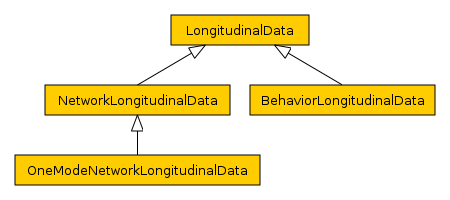
\includegraphics[scale=.5]{LongitudinalData.png}
\end{center}
The base class \nnm{LongitudinalData} is not supposed to
be created directly, however, it provides some useful methods applicable to
observed data of all types of dependent variables:
\begin{itemize}
\item \verb|const| \nnm{ActorSet} * \nnm{pActorSet}() -- returns the set of
actors this dependent variable is defined for.
\item \verb|int| \nnm{n}() -- returns the size of the set of actors.
\item \verb|int| \nnm{observationCount}() -- returns the number of observations
that can be stored in this data object.
\item \verb|bool| \nnm{upOnly}(\verb|int| \nnm{period}) -- returns if only
upward changes are observed in the given period.
\item \verb|void| \nnm{upOnly}(\verb|int| \nnm{period}, \verb|bool| \nnm{flag})
-- stores the indicator if only upward changes are observed in the given period.
Note that the \nnm{LongitudinalData} class provides just the storage of these
flags, and their values have to be computed elsewhere. They are currently
passed in from the R part of the system.
\item \nnm{downOnly} -- similar accessor methods for flags indicating that only
downward changes are observed.
\end{itemize}

The derived classes of \nnm{LongitudinalData} are created with the factory
methods of the \nnm{Data} class by providing the name of the variable and
the corresponding actor set (or both the set of tie senders and the set of
tie receivers in the case of two-mode networks):
\begin{itemize}
\item one-mode networks
\begin{verbatim}
OneModeNetworkLongitudinalData * pFriendshipData =
  pData->createOneModeNetworkData("friendship",
    pStudents);
\end{verbatim}
\item two-mode networks
\begin{verbatim}
NetworkLongitudinalData * pCourseSelectionData =
  pData->createNetworkData("courses",
    pStudents,
    pCourses);
\end{verbatim}
\item behavior
\begin{verbatim}
BehaviorLongitudinalData * pAverageGradeData =
  pData->createBehaviorData("grade", pStudents);
\end{verbatim}
\end{itemize}

\subsubsection{Two-Mode Network Variables}

\paragraph{Network Structure.}

The main purpose of the \nnm{NetworkLongitudinalData} class is to store the
values of network ties in each of the observations as well as indicators about
whether a tie value is missing or structurally determined. This can be done with
the following setter methods:
\begin{itemize}
\item \verb|void| \nnm{tieValue}(\verb|int| \nnm{i}, \verb|int| \nnm{j},
\verb|int| \nnm{observation}, \verb|int| \nnm{value}) -- stores the value of
the tie between the given actors at the given observation,
\item \verb|void| \nnm{missing}(\verb|int| \nnm{i}, \verb|int| \nnm{j},
\verb|int| \nnm{observation}, \verb|bool| \nnm{flag}) -- stores if the value of
the tie between the given actors is missing at the given observation,
\item \verb|void| \nnm{structural}(\verb|int| \nnm{i}, \verb|int| \nnm{j},
\verb|int| \nnm{observation}, \verb|bool| \nnm{flag}) -- stores if the value of
the tie between the given actors is structurally determined at the given
observation.
\end{itemize}

There is a corresponding set of methods for accessing the stored values:
\begin{itemize}
\item \verb|int| \nnm{tieValue}(\verb|int| \nnm{i}, \verb|int| \nnm{j},
\verb|int| \nnm{observation})
\item \verb|bool| \nnm{missing}(\verb|int| \nnm{i}, \verb|int| \nnm{j},
\verb|int| \nnm{observation})
\item \verb|bool| \nnm{structural}(\verb|int| \nnm{i}, \verb|int| \nnm{j},
\verb|int| \nnm{observation})
\end{itemize}

Internally, this information is stored in three arrays of networks, namely,
\nnm{lnetworks} for the observed tie values, \nnm{lmissingTieNetworks} for
indicators of missing ties, and \nnm{lstructuralTieNetworks} for storing the
indicators of structurally determined ties. To enable effective iteration over
all ties, the class \nnm{NetworkLongitudinalData} provides constant access to
these networks via the following methods:
\begin{itemize}
\item \verb|const| \nnm{Network} * \nnm{pNetwork}(\verb|int| \nnm{observation})
-- returns the network of observed values at the given observation,
\item \verb|const| \nnm{Network} *
\nnm{pMissingTieNetwork}(\verb|int| \nnm{observation}) -- returns the network of
missing tie indicators for the given observation,
\item \verb|const| \nnm{Network} *
\nnm{pStructuralTieNetwork}(\verb|int| \nnm{observation}) -- returns the network
of structural tie indicators for the given observation.
\end{itemize}

For example, the following code snippets demonstrate two ways of iterating over
the selected courses of a certain student $i$, but the second snippet is much
more efficient.

\emph{Example 1}
\begin{verbatim}
for (int j = 0; j < pCourses->n(); j++)
{
  if (pCourseSelectionData->tieValue(i, j, observation) != 0)
  {
    cout << "The student " << i <<
      " has selected the course " << j << endl;
  }
}
\end{verbatim}

\emph{Example 2}
\begin{verbatim}
const Network * pNetwork =
  pCourseSelectionData->pNetwork(observation);

IncidentTieIterator iter = pNetwork->outTies(i);

while (iter.valid())
{
  int j = iter.actor();
  cout << "The student " << i <<
    " has selected the course " << j << endl;
  iter.next();
}
\end{verbatim}

\paragraph{Calculating Properties.}

Once a network data object has been populated, it is important to call the
\nnm{calculateProperties} method that computes important properties of the
observed data, which are used by some effects during model simulations:
\begin{verbatim}
pCourseSelectionData->calculateProperties();

cout << "The average number of courses per student is " <<
  pCourseSelectionData->averageOutDegree() << endl;
cout << "The average number of students " <<
  "attending a course is " <<
  pCourseSelectionData->averageInDegree() << endl;
\end{verbatim}

\paragraph{Other Methods.}
\begin{itemize}
\item \verb|void| \nnm{maxDegree}(\verb|int| \nnm{degree}) -- if there is a
restriction on the maximum number of outgoing ties an actor can have, it has
to be specified by using this method.
\end{itemize}

\subsubsection{One-Mode Network Variables}

Since one-mode networks are a special kind of two-mode networks, the class
\nnm{OneModeNetworkLongitudinalData} derives from \nnm{NetworkLongitudinalData}
and inherits all its methods. The derived class provides some additional
methods, though, which are applicable to one-mode networks only:
\begin{itemize}
\item \verb|void| \nnm{symmetric}(\verb|bool| \nnm{flag}) -- stores if the
network is symmetric,
\item \verb|void| \nnm{balanceMean}(\verb|double| \nnm{value}) -- stores the
centering constant for the balance effect.
\end{itemize}
Some of the information that is simply stored in the
\nnm{OneModeNetworkLongitudinalData} class could be computed by the class
itself, but since this information is already computed in R, we save the effort
of computing it again, and simply pass the values in from the R part of the
system.

\subsubsection{Behavior Variables}

Analogous to the data class for network variables, the class
\nnm{BehaviorLongitudinalData} stores the observed values of a certain behavior
variable and various properties computed from the observed data.

\paragraph{Observed Values.}
The observed values or indications about missing values can be stored with the
following methods:
\begin{itemize}
\item \verb|void| \nnm{value}(\verb|int| \nnm{observation},
\verb|int| \nnm{actor}, \verb|int| \nnm{value})
\item \verb|void| \nnm{missing}(\verb|int| \nnm{observation},
\verb|int| \nnm{actor}, \verb|bool| \nnm{missing})
\end{itemize}

The stored values can be accessed with these methods:
\begin{itemize}
\item \verb|int| \nnm{value}(\verb|int| \nnm{observation},
\verb|int| \nnm{actor})
\item \verb|bool| \nnm{missing}(\verb|int| \nnm{observation},
\verb|int| \nnm{actor})
\end{itemize}

Internally, the observed values are stored in an $M \times N$ integer array
\nnm{lvalues} and the missingness indicators are stored in an $M \times N$
boolean array \nnm{lmissing}, where $M$ is the number of observations and $N$ is
the number of actors in the corresponding actor set. A read-only access to a
whole row of the matrix of values (namely, the values of all actors in a single
observation) is provided by the method
\begin{itemize}
\item \verb|const| \verb|int| * \nnm{values}(\verb|int| \nnm{observation}).
\end{itemize}

\paragraph{Calculating Properties.} 
Again, as soon as the observed values and missingness indicators are stored, and
before the data object can be used for model simulations, the method
\nnm{calculateProperties} should be called:
\begin{verbatim}
pAverageGradeData->calculateProperties();

cout << "The average grades of students range from " <<
  pAverageGradeData->min() << " to " <<
  pAverageGradeData->max() << endl;
\end{verbatim}
The method \nnm{calculateProperties} calculates some properties of the
observed data, which can be subsequently queried with the following methods:
\begin{itemize}
\item \verb|int| \nnm{min}() -- returns the smallest observed non-missing value,
\item \verb|int| \nnm{max}() -- returns the largest observed non-missing value,
\item \verb|int| \nnm{range}() -- returns the range of observed non-missing
values, which is simply the difference between the maximum and the minimum
values,
\item \verb|double| \nnm{overallMean}() -- returns the overall mean of the
observed non-missing values defined as
$\frac{1}{M}\sum_{k=1}^{M} \frac{\sum_{i \in A_k} v_i^k}{|A_k|}$, where $v_i^k$
is the observed behavior for actor $i$ and the observation $k$ and $A_k$ is the
set of actors with non-missing values at the observation $k$.
\end{itemize}

\paragraph{Other Methods.}
\begin{itemize}
\item \verb|void| \nnm{similarityMean}(\verb|double| \nnm{similarityMean}) --
stores the mean similarity of actor behavior values over all
observations, which is calculated in R.
\item \verb|double| \nnm{similarity}(\verb|double| \nnm{a},
\verb|double| \nnm{b}) -- returns the centered similarity score for the given
values $a$ and $b$. The similarity score is defined as
$1 - \frac{|a-b|}{\Delta}$, where $\Delta$ is the observed range of the
behavior variable, and the mean similarity is subtracted from this expression to
obtain the centered similarity score.
\end{itemize}

\subsection{Covariates}
The classes for storing actor covariates and dyadic covariates are organised in
two separate hierarchies:
\begin{center}
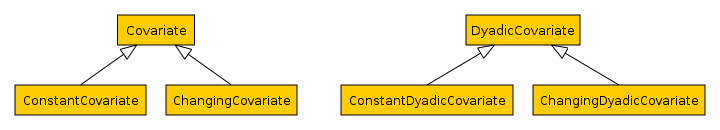
\includegraphics[scale=.5]{Covariates.png}
\end{center}
Since the usage of covariate classes is very similar to that of observed data
for behavior variables, we will just briefly list the main methods for working
with covariates.

The covariate data classes can be created by the factory methods of the
\nnm{Data} class:
\begin{itemize}
\item \nnm{ConstantCovariate} * \nnm{createConstantCovariate}(\ldots)
\item \nnm{ChangingCovariate} * \nnm{createChangingCovariate}(\ldots)
\item \nnm{ConstantDyadicCovariate} *
\nnm{createConstantDyadicCovariate}(\ldots)
\item \nnm{ChangingDyadicCovariate} *
\nnm{createChangingDyadicCovariate}(\ldots)
\end{itemize}
The name of the covariate and one (for actor covariates) or two (for dyadic
covariates) actor sets should be provided as parameters for these methods.

\subsubsection{Actor Covariates}
The base class \nnm{Covariate} for actor covariates provides the following
methods:
\begin{itemize}
\item \verb|void| \nnm{range}(\verb|double| \nnm{range}) -- stores the observed
range of the covariate. Unlike the observed data for behavior variables, it is
not computed by the covariate class itself, but passed in from R.
\item \verb|double| \nnm{range}() -- returns the observed range of the
covariate.
\item \nnm{similarityMean}(\ldots) and \nnm{similarity}(\ldots) -- these methods
behave precisely as the corresponding methods in the
\nnm{BehaviorLongitudinalData} class.
\end{itemize}

The derived classes \nnm{ConstantCovariate} and \nnm{ChangingCovariate} provide
appropriate methods \nnm{value}(\ldots) and \nnm{missing}(\ldots) for storing
and retrieving the values of the covariate and the missingness indicators,
respectively. Internally, the data is stored in one-dimensional or
two-dimensional $N \times M$ arrays \nnm{lvalues} and \nnm{lmissing}, where
$N$ is the number of actors in the respective set and $M$ is the number of
observations.

\subsubsection{Dyadic Covariates}
The interface of the dyadic covariates is very similar to that of actor
covariates and should not present any difficulties. The base class
\nnm{DyadicCovariate} provides access to both relevant sets of actors (methods
\nnm{pFirstActorSet}() and \nnm{pSecondActorSet}()) and a storage of the mean
value of the covariate that is passed in from R (\nnm{mean}(\ldots) methods).

Again, the values of the covariate and their missingness indicators can be
stored and accessed with methods \nnm{value}(\ldots) and \nnm{missing}(\ldots),
which are defined in the derived classes \nnm{ConstantDyadicCovariate} and
\nnm{ChangingDyadicCovariate}.

The internal representation of the values is tricky, though. Since storing
a sparse $N_1 \times N_2$ (the sizes of both involved actor sets) matrix
explicitly is expensive in terms of memory, we store each row of the matrix
as an instance of \nnm{map}$<$\verb|int|, \verb|double|$>$ that maps
each column index with a non-zero value in that row to the respective value.
The matrix of missings has only 0 and 1 as its entries, so an instance of
\nnm{set}$<$\verb|int|$>$ is more appropriate for storing the column indices
with missings in a certain row. Array of such maps or sets (like
\nnm{lpRowValues} and \nnm{lpRowMissings} in \nnm{ConstantDyadicCovariate}),
one for each row, then represents the whole matrices. Such a representation is
not only space-efficient, but also suitable for fast iteration over non-zero
values in a certain row. To facilitate an equally fast iteration over non-zero
values in a certain column, we maintain analogous structures for columns in
\nnm{lpColumnValues} and \nnm{lpColumnMissings}. The following methods in
\nnm{ConstantDyadicCovariate} exploit
this internal representation to provide fast iterators over non-zero non-missing
values of in a given row or column:
\begin{itemize}
\item \nnm{DyadicCovariateValueIterator} \nnm{rowValues}(\verb|int| \nnm{i})
\item \nnm{DyadicCovariateValueIterator} \nnm{columnValues}(\verb|int| \nnm{j})
\end{itemize}
%
\emph{Example}

The following example multiplies the row $i$ with the column $j$.
\begin{verbatim}
DyadicCovariateValueIterator rowIter =
  pCovariate->rowValues(i);
DyadicCovariateValueIterator columnIter =
  pCovariate->columnValues(j);

double product = 0;

while (rowIter.valid() && columnIter.valid())
{
  if (rowIter.actor() < columnIter.actor())
  {
    rowIter.next();
  }
  else if (rowIter.actor() > columnIter.actor())
  {
    columnIter.next();
  }
  else
  {
    product += rowIter.value() * columnIter.value();
    rowIter.next();
    columnIter.next();
  }
}
\end{verbatim}

Finally, we should note that the \nnm{ChangingDyadicCovariate} class has the
same functionality as discussed above for constant dyadic covariates, except
that the methods expect the observation to be specified as an additional
parameter and that the dimensionality of the whole storage increases by one.

\subsection{Composition Change}

If a set of actors is not constant over time because actors join or leave, it
has to be specified in the \nnm{Data} object. The following methods of the
\nnm{Data} class should be used for this purpose:
\begin{itemize}
\item \verb|void| \nnm{active}(\verb|const| \nnm{ActorSet} * \nnm{pActorSet},\\
\verb|  int| \nnm{actor},\\
\verb|  int| \nnm{observation},\\
\verb|  bool| \nnm{flag}) -- specifies if the given actor of the given set of
actors is active at the given observation.
\item \verb|void| \nnm{addJoiningEvent}(\verb|int| \nnm{period},\\
\verb|  const| \nnm{ActorSet} * \nnm{pActorSet},\\
\verb|  int| \nnm{actor},\\
\verb|  double| \nnm{time}) -- stores the time of a period when an actor joins
a certain actor set.
\item \verb|void| \nnm{addLeavingEvent}(\verb|int| \nnm{period},\\
\verb|  const| \nnm{ActorSet} * \nnm{pActorSet},\\
\verb|  int| \nnm{actor},\\
\verb|  double| \nnm{time}) -- stores the time of a period when an actor leaves
a certain actor set.
\end{itemize}
The time values in the above methods have to lie in the range $[0,1]$ with
values 0 and 1 representing the start and end point of the period, respectively.
For example, assuming that the length of a period is one year, the following
code snippet expresses the fact that and the student $i$ leaves the university 3
months after the second observation and resumes the studies half year after the
third observation (remember that the indices of observations start with 0):
\begin{verbatim}
for (int k = 0; k < observationCount; k++)
{
  if (k == 2)
  {
    pData->active(pStudents, i, k, false);
  }
  else
  {
    // This is not strictly necessary,
    // as the actors are active by default

    pData->active(pStudents, i, k, true);
  }
}

pData->addLeavingEvent(1, pStudents, i, .25);
pData->addJoiningEvent(2, pStudents, i, .5);
\end{verbatim}

The details about every exogenous event are collected in instances of the
\nnm{ExogenousEvent} class, which are stored in sets of type \nnm{EventSet},
one for each period. These sets can be accessed with the method
\nnm{pEventSet}(\verb|int|~\nnm{period}).

\subsection{Accessor Methods}

Once a \nnm{Data} object has been populated, its sub-objects can be accessed
in two ways. A single object can be looked up by its name, like in the following
examples.
\begin{verbatim}
const ActorSet * pStudents = pData->pActorSet("students");
OneModeNetworkLongitudinalData * pFriendshipData =
  pData->pOneModeNetworkData("friendship");
\end{verbatim}
If some operation is to be performed for all sub-objects of a certain type, one
can obtain a reference to the vector, where the subobjects of this type are
stored by the \nnm{Data} class. For example, the values of all constant
covariates can be printed as follows:
\begin{verbatim}
const vector<ConstantCovariate *> & rCovariates =
  pData->rConstantCovariates();

for (unsigned i = 0; i < rCovariates.size(); i++)
{
  ConstantCovariate * pCovariate = rCovariates[i];

  cout << pCovariate->name() << endl;

  for (int j = 0; j < pCovariate->pActorSet()->n(); j++)
  {
    cout << j << " " << pCovariate->value(j) << endl;
  }
}
\end{verbatim}

\section{Models}

\end{document}
